% Wishlist of things to cover
% Wikipedia as source for equations


\documentclass{beamer}
%
% Choose how your presentation looks.
%
% For more themes, color themes and font themes, see:
% http://deic.uab.es/~iblanes/beamer_gallery/index_by_theme.html
%

% Theme License: https://creativecommons.org/licenses/by/4.0/

\mode<presentation>
{
  \usetheme{metropolis}   % https://github.com/matze/mtheme
  \usecolortheme{default} % or try albatross, beaver, crane, ...
  \usefonttheme{default}  % or try serif, structurebold, ...
  \setbeamertemplate{navigation symbols}{}
  %% \setbeamertemplate{caption}[numbered]
  \setbeamertemplate{caption}{\raggedright\insertcaption\par}
}

\usepackage[english]{babel}
\usepackage[utf8x]{inputenc}

\title{An Introduction to \LaTeX}
\author{Jake Vossen}
\institute{Colorado School of Mines - acm-w}
\date{2020-02-26}

\begin{document}
\begin{frame}{Something to consider...}
    \begin{figure}
    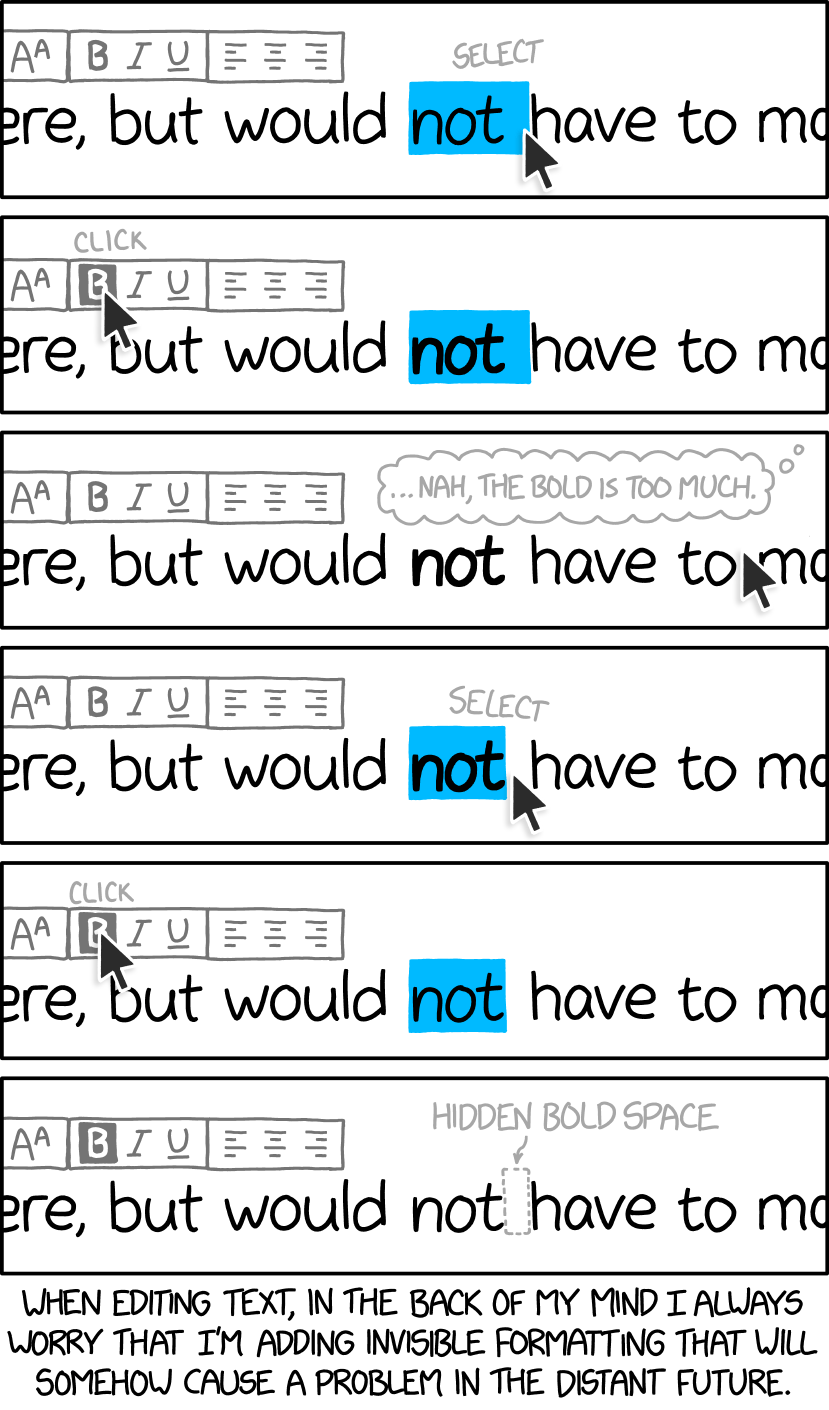
\includegraphics[scale=.13]{invisible_formatting_2x.png}
    \caption{https://xkcd.com/2109/}
  \end{figure}
\end{frame}
\begin{frame}
  \titlepage
\end{frame}

% Uncomment these lines for an automatically generated outline.
%\begin{frame}{Outline}
%  \tableofcontents
%\end{frame}

\section{What is \LaTeX?}

\begin{frame}[fragile]
  \frametitle{What is \LaTeX}

  It is \textbf{not} a ``what you see is what you get'' editor (WYSIWYG)

  %% text
\begin{verbatim}
  \begin{equation}
        x = \frac{ - b \pm \sqrt{b^2 - 4 a c}}{2a}
  \end{equation}
\end{verbatim}
\par
  \hrulefill\par
%% \hline
  \begin{equation}
        x = \frac{ - b \pm \sqrt{b^2 - 4 a c}}{2a}
  \end{equation}

\end{frame}

\begin{frame}[fragile]
\frametitle{More \LaTeX}
\begin{verbatim}
\begin{equation}
  \int_0^a x^n dx = \frac{1}{n+1}\
  a^{n+1} \qquad n \geq 0
\end{equation}
\end{verbatim}\par
  \hrulefill\par

\begin{equation}
  \int_0^a x^n dx = \frac{1}{n+1}\
  a^{n+1} \qquad n \geq 0
\end{equation}

\end{frame}

\section{The Why}


\begin{frame}{Widespread use in Academia}

  \begin{enumerate}
    \item {Almost all journals, especially in Math, CS, and Physics
      either prefer or mandate \LaTeX as the document submission
      format}
   \end{enumerate}

\vskip 1cm

\end{frame}

\begin{frame}{Formatting of Equations}


\vskip 1cm

\end{frame}

\begin{frame}{Faster Equation Creation (maybe after some initial costs)}


\end{frame}

\begin{frame}[fragile]
  \frametitle{Better looking equations (arguably)}

  \begin{itemize}

  \item{Word}

  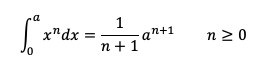
\includegraphics[scale=.75]{word-equation.png}

  \item{\LaTeX}

  \begin{equation}
  \int_0^a x^n dx = \frac{1}{n+1}\
  a^{n+1} \qquad n \geq 0
  \end{equation}

  \end{itemize}

\end{frame}


\begin{frame}{Tooling}

  % Git, text editors, etc
\end{frame}


\end{document}
